\documentclass[tikz,border=8pt]{standalone}
\usepackage{amsmath,amssymb}
\usepackage{tikz}
\usetikzlibrary{arrows.meta,calc,decorations.pathreplacing,patterns,shapes.geometric,positioning,shadings,decorations.pathmorphing}

\begin{document}
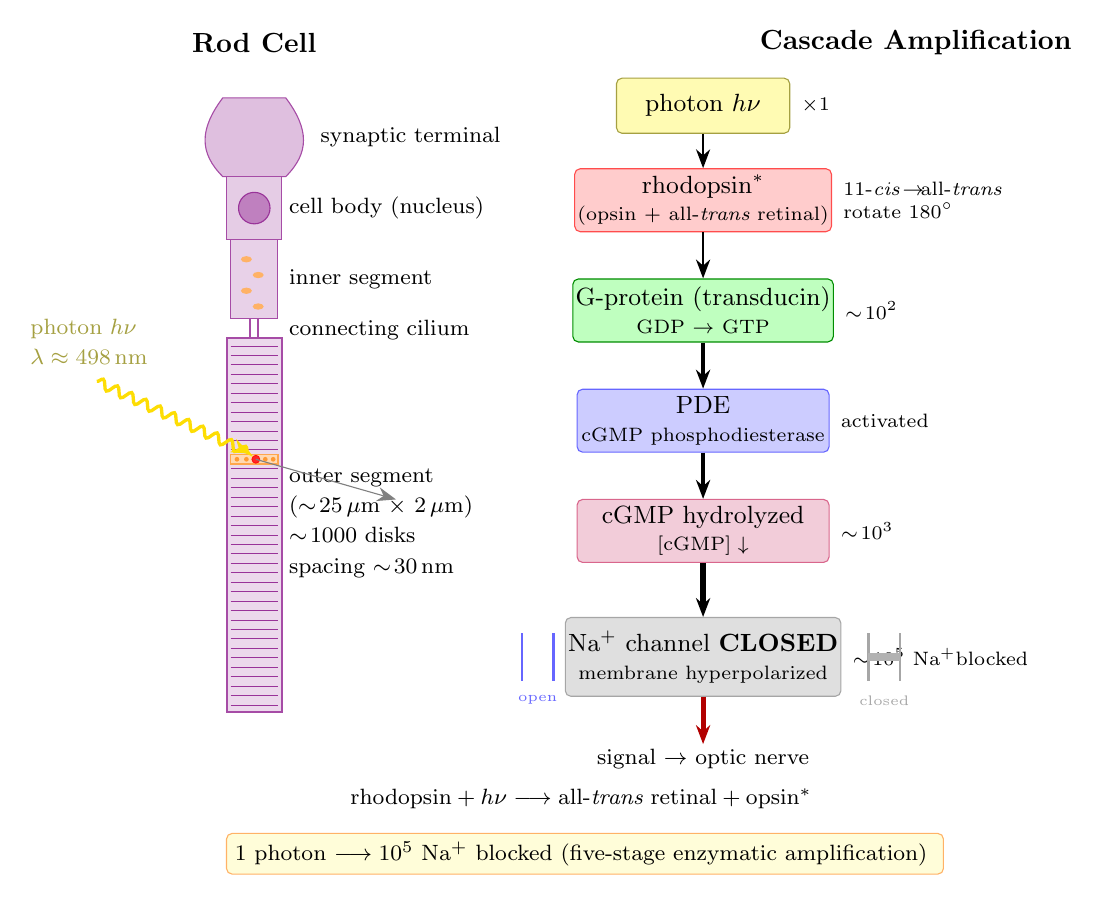
\begin{tikzpicture}[
  font=\small,
  >={Stealth[length=2.4mm]},
  every node/.style={inner sep=1pt}
]

% ============================================================
% LEFT PANEL: rod cell longitudinal cross-section
% ============================================================

% Rod cell label
\node[font=\bfseries] at (-5.2,5.3) {Rod Cell};

% Synaptic terminal (top)
\fill[violet!25] (-5.6,4.6) .. controls (-5.9,4.2) and (-5.9,3.9) .. (-5.6,3.6)
  -- (-4.8,3.6) .. controls (-4.5,3.9) and (-4.5,4.2) .. (-4.8,4.6) -- cycle;
\draw[violet!70] (-5.6,4.6) .. controls (-5.9,4.2) and (-5.9,3.9) .. (-5.6,3.6)
  -- (-4.8,3.6) .. controls (-4.5,3.9) and (-4.5,4.2) .. (-4.8,4.6) -- cycle;
\node[right] at (-4.4,4.1) {\footnotesize synaptic terminal};

% Cell body with nucleus
\fill[violet!20] (-5.55,3.6) rectangle (-4.85,2.8);
\draw[violet!70] (-5.55,3.6) rectangle (-4.85,2.8);
\fill[violet!50] (-5.2,3.2) circle (0.2);
\draw[violet!80] (-5.2,3.2) circle (0.2);
\node[right] at (-4.8,3.2) {\footnotesize cell body (nucleus)};

% Inner segment
\fill[violet!18] (-5.5,2.8) rectangle (-4.9,1.8);
\draw[violet!70] (-5.5,2.8) rectangle (-4.9,1.8);
\node[right] at (-4.8,2.3) {\footnotesize inner segment};
% Mitochondria hints
\fill[orange!60] (-5.3,2.55) ellipse (0.07 and 0.04);
\fill[orange!60] (-5.15,2.35) ellipse (0.07 and 0.04);
\fill[orange!60] (-5.3,2.15) ellipse (0.07 and 0.04);
\fill[orange!60] (-5.15,1.95) ellipse (0.07 and 0.04);

% Connecting cilium
\draw[violet!70,thick] (-5.25,1.8) -- (-5.25,1.55);
\draw[violet!70,thick] (-5.15,1.8) -- (-5.15,1.55);
\node[right] at (-4.8,1.65) {\footnotesize connecting cilium};

% Outer segment container
\fill[violet!15] (-5.55,1.55) rectangle (-4.85,-3.2);
\draw[violet!70,thick] (-5.55,1.55) rectangle (-4.85,-3.2);
\node[right,align=left] at (-4.8,-0.8)
  {\footnotesize outer segment\\\footnotesize ($\sim\!25\,\mu$m $\times$ 2\,$\mu$m)\\\footnotesize $\sim\!1000$ disks\\\footnotesize spacing $\sim\!30$\,nm};

% Disks (stacked)
\foreach \y in {1.45,1.33,1.21,1.09,0.97,0.85,0.73,0.61,0.49,0.37,0.25,0.13,0.01,-0.11,-0.23,-0.35,-0.47,-0.59,-0.71,-0.83,-0.95,-1.07,-1.19,-1.31,-1.43,-1.55,-1.67,-1.79,-1.91,-2.03,-2.15,-2.27,-2.39,-2.51,-2.63,-2.75,-2.87,-2.99,-3.11}{
  \draw[violet!80,line width=0.25pt] (-5.5,\y) -- (-4.9,\y);
}

% Highlighted disk (where photon hits) with rhodopsin molecules
\fill[orange!30] (-5.5,-0.05) rectangle (-4.9,0.07);
\draw[orange!70,line width=0.5pt] (-5.5,-0.05) rectangle (-4.9,0.07);
% Rhodopsin molecules on the disk (tiny circles)
\foreach \x in {-5.42,-5.3,-5.18,-5.06,-4.96}{
  \fill[orange!80] (\x,0.01) circle (0.03);
}
% Activated one
\fill[red!85] (-5.18,0.01) circle (0.05);
\draw[red!95,line width=0.3pt] (-5.18,0.01) circle (0.05);

% Incoming photon (yellow wavy arrow)
\draw[yellow!80!orange,line width=1.2pt,decorate,decoration={snake,amplitude=0.6mm,segment length=2mm},->]
  (-7.2,1.0) -- (-5.25,0.08);
\node[yellow!60!black,align=left] at (-7.3,1.5)
  {\footnotesize photon $h\nu$\\\footnotesize $\lambda \approx 498$\,nm};

% Label on activated rhodopsin
\draw[->,thin,gray] (-5.18,0.01) -- (-3.4,-0.5);

% ============================================================
% RIGHT PANEL: cascade chain
% ============================================================

\node[font=\bfseries] at (3.2,5.3) {Cascade Amplification};

% Stage 1: Photon
\node[draw=yellow!60!black,fill=yellow!30,rounded corners=2pt,minimum width=2.2cm,minimum height=0.7cm] (ph) at (0.5,4.5) {photon $h\nu$};
\node[right=0.1cm of ph,font=\scriptsize] {$\times 1$};

% Stage 2: Rhodopsin (activated)
\node[draw=red!70,fill=red!20,rounded corners=2pt,minimum width=2.8cm,minimum height=0.8cm,align=center] (rh) at (0.5,3.3)
  {rhodopsin$^{*}$\\[-1pt]\scriptsize (opsin + all-$\textit{trans}$ retinal)};
\node[right=0.1cm of rh,font=\scriptsize,align=left] {11-$\textit{cis}\!\to\!$all-$\textit{trans}$\\rotate $180^{\circ}$};

% Stage 3: Transducin (G-protein)
\node[draw=green!55!black,fill=green!25,rounded corners=2pt,minimum width=3.2cm,minimum height=0.8cm,align=center] (gp) at (0.5,1.9)
  {G-protein (transducin)\\[-1pt]\scriptsize GDP $\to$ GTP};
\node[right=0.1cm of gp,font=\scriptsize] {$\sim\!10^{2}$};

% Stage 4: PDE
\node[draw=blue!60,fill=blue!20,rounded corners=2pt,minimum width=3.2cm,minimum height=0.8cm,align=center] (pde) at (0.5,0.5)
  {PDE\\[-1pt]\scriptsize cGMP phosphodiesterase};
\node[right=0.1cm of pde,font=\scriptsize] {activated};

% Stage 5: cGMP hydrolysis
\node[draw=purple!60,fill=purple!20,rounded corners=2pt,minimum width=3.2cm,minimum height=0.8cm,align=center] (cg) at (0.5,-0.9)
  {cGMP hydrolyzed\\[-1pt]\scriptsize $[\mathrm{cGMP}]\downarrow$};
\node[right=0.1cm of cg,font=\scriptsize] {$\sim\!10^{3}$};

% Stage 6: Na+ channel closed
\node[draw=gray!70,fill=gray!25,rounded corners=2pt,minimum width=3.4cm,minimum height=1.0cm,align=center] (na) at (0.5,-2.5)
  {Na$^{+}$ channel \textbf{CLOSED}\\[-1pt]\scriptsize membrane hyperpolarized};
\node[right=0.1cm of na,font=\scriptsize] {$\sim\!10^{5}$ Na$^{+}$\\blocked};

% Door-like channel symbols (open vs closed)
% Open channel (small, on left of na box)
\begin{scope}[shift={(-1.6,-2.5)}]
  \draw[thick,blue!60] (-0.2,-0.3) -- (-0.2,0.3);
  \draw[thick,blue!60] (0.2,-0.3) -- (0.2,0.3);
  \node[font=\tiny,blue!60] at (0,-0.55) {open};
\end{scope}
% Closed channel
\begin{scope}[shift={(2.8,-2.5)}]
  \draw[thick,gray!70] (-0.2,-0.3) -- (-0.2,0.3);
  \draw[thick,gray!70] (0.2,-0.3) -- (0.2,0.3);
  \fill[gray!60] (-0.2,-0.05) rectangle (0.2,0.05);
  \node[font=\tiny,gray!70] at (0,-0.55) {closed};
\end{scope}

% Arrows between stages (gradually thickening)
\draw[->,line width=0.5pt] (ph) -- (rh);
\draw[->,line width=0.9pt] (rh) -- (gp);
\draw[->,line width=1.3pt] (gp) -- (pde);
\draw[->,line width=1.7pt] (pde) -- (cg);
\draw[->,line width=2.2pt] (cg) -- (na);

% Signal out arrow
\draw[->,line width=1.8pt,red!70!black] (na.south) -- ++(0,-0.6) node[below,font=\footnotesize,black] {signal $\to$ optic nerve};

% ============================================================
% Bottom summary equation / caption
% ============================================================
\node[align=center,font=\footnotesize] at (-1.0,-4.3) {
  $\mathrm{rhodopsin} + h\nu \longrightarrow \mathrm{all\text{-}}\textit{trans}\ \mathrm{retinal} + \mathrm{opsin}^{*}$
};
\node[align=center,font=\footnotesize,fill=yellow!15,draw=orange!60,rounded corners=2pt,inner sep=3pt] at (-1.0,-5.0) {
  $1$ photon $\longrightarrow 10^{5}$ Na$^{+}$ blocked (five-stage enzymatic amplification)
};

\end{tikzpicture}
\end{document}
